% fig12_gate_status — non-wet-lab gate status (orange/green/white).
% Standalone pgfplots; compiled to figures/fig12_gate_status.pdf.
% Comparison (gate status counts) => chart (user hard rule).
% Data: Appendix J, UFO/verify/V4_tier_ledger.md §3:
%   2 orange unconverged (CFD, circle-arrow), 4 green closed
%   (EM/FEA/thermal/F-ANTI-3), 13 white open (Stage-4-7 falsifiers).
\documentclass[border=4pt]{standalone}
\usepackage{tikz}
\usepackage{pgfplots}
\pgfplotsset{compat=1.18}
\begin{document}
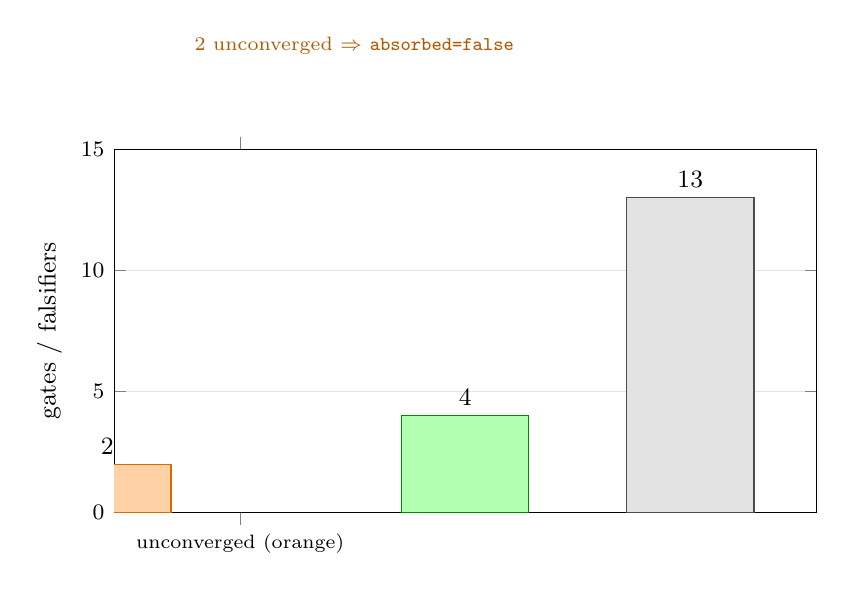
\begin{tikzpicture}
\begin{axis}[
  width=10.5cm, height=6.2cm,
  ybar,
  bar width=46pt,
  ymin=0, ymax=15,
  ylabel={gates / falsifiers},
  symbolic x coords={{unconverged (orange)}, {closed (green)}, {open (white)}},
  xtick=data,
  x tick label style={font=\scriptsize},
  tick label style={font=\footnotesize},
  label style={font=\small},
  nodes near coords,
  nodes near coords style={font=\small},
  ymajorgrids, grid style={gray!22},
  enlarge x limits=0.28,
]
\addplot[draw=orange!85!black,fill=orange!35] coordinates {({unconverged (orange)},2)};
\addplot[draw=green!55!black,fill=green!30, bar shift=0pt] coordinates {({closed (green)},4)};
\addplot[draw=gray!60!black,fill=gray!22, bar shift=0pt] coordinates {({open (white)},13)};
\end{axis}
\node[font=\scriptsize, orange!70!black, anchor=south west] at (0.9cm,5.7cm)
  {2 unconverged $\Rightarrow$ \texttt{absorbed=false}};
\end{tikzpicture}
\end{document}
